\chapter{Introduction}
\label{sec:intro}

% Die Einleitung schreibt man zuletzt, wenn die Arbeit im Großen und
% Ganzen schon fertig ist. (Wenn man mit der Einleitung beginnt - ein
% häufiger Fehler - braucht man viel länger und wirft sie später doch
% wieder weg). Sie hat als wesentliche Aufgabe, den Kontext für die
% unterschiedlichen Klassen von Lesern herzustellen. Man muß hier die
% Leser für sich gewinnen. Das Problem, mit dem sich die Arbeit befaßt,
% sollte am Ende wenigsten in Grundzügen klar sein und dem Leser
% interessant erscheinen. Das Kapitel schließt mit einer Übersicht über
% den Rest der Arbeit. Meist braucht man mindestens 4 Seiten dafür, mehr
% als 10 Seiten liest keiner.


% \section{A Section}

% Referencing other chapters: \ref{sec:state} \ref{sec:design}
% \ref{sec:implementation} \ref{sec:evaluation} \ref{sec:futurework}
% \ref{sec:conclusion}

% \begin{table}[htp]
%   \centering
%   \begin{tabular}{lrr}
%     \textbf{Name} & \textbf{Y} & \textbf{Z} \\
%     \hline
%     \textit{Foo} & 20,614 & \unit[23]{\%} \\
%     \textit{Bar} & 9,914 & \unit[11]{\%} \\
%     \textit{Foo + Bar} & 30,528 & \unit[34]{\%} \\
%     \hline
%     \textit{total} & 88,215 & \unit[100]{\%} \\

%   \end{tabular}
%   \caption[Some interesting numbers]{Various very important looking numbers and sums.}
%   \label{tab:numbers}
% \end{table}

% More text referencing Table~\ref{tab:numbers}.

% \section{Another Section}

% \begin{figure}[tbp]
%   \centering
%   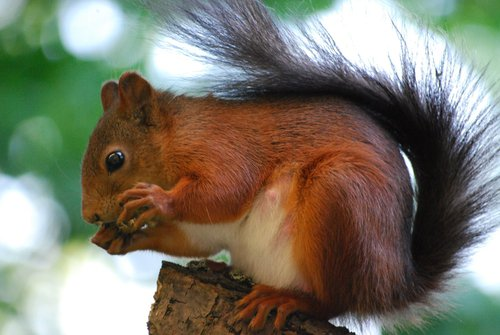
\includegraphics[width=0.8\textwidth]{images/squirrel}
%   \caption[Short description]{A long description of this squirrel figure.
%   Image taken from
%   \url{http://commons.wikimedia.org/wiki/File:Sciurus-vulgaris_hernandeangelis_stockholm_2008-06-04.jpg}}
%   \label{fig:squirrel}
% \end{figure}

% Citing \cite{bellard2005qfa} other documents \cite{bellard2005qfa, boileau06}
% and Figure~\ref{fig:squirrel}.

% Something with umlauts and a year/month date:
% \cite{becher04:_feurig_hacken_mit_firew}.

% And some online resources: \cite{green04}, \cite{patent:4819234}

% \section{Yet Another Section}

% \todo{add content}

% \begin{figure}[tbp]
%  \missingfigure{Come up with a mindblowing figure.}
%  \caption{A mindblowing figure}
%  \label{fig:todo}
% \end{figure}

% \section{Test commands}

% \drops \LLinux \NOVA \QEMU
% \texttt{memcpy}
% A sentence about BASIC. And a correctly formatted one about ECC\@.



With the popularization of new generation hardware on the network and storage, the processing speed 
of data packets on the hardware is getting faster and faster\cite{12}. For example, 
the bandwidth of the smart
network card has reached 100Gb/s. Under this circumstance, the traditional perception
 that the packet processing speed on hardware is lower than the packet processing speed in 
 software is overturned\cite{Ousterhout1990WhyAO}, i.e.,
The software has become a performance bottleneck in data transmission.
The reason is obvious. Compared with the continuous upgrading of hardware, 
the communication between the application and the device still relies 
on the kernel IO stack. 

\begin{figure}[H]
  \centering
  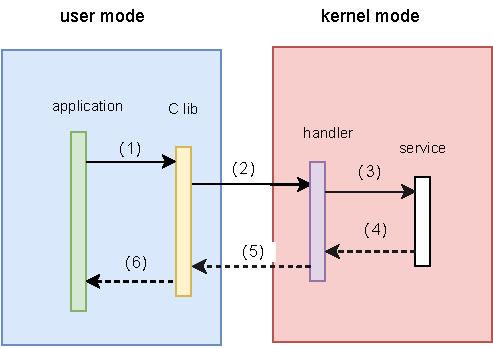
\includegraphics[width=0.8\textwidth]{images/system_call}
  \caption[System Call Process]{System Call Process}
  \label{fig:system_call_process}
\end{figure}
 
Typically, IO operations are performed via system calls, 
which build a bridge between applications and the devices.  
 On a 32-bit system, an application leverages the int80 
interrupt to trigger system calls. This method is slow because it is not designed explicitly for system calls. 
The CPU must check the interrupt descriptor table placed on the memory before handling the interrupt. Due to
 the cost of memory operations, on the 64-bit system, new instructions \emph{SYSCALL}/\emph{SYSRET} for system 
 call entering to and existing from the kernel are introduced. The CPU can employ those new instructions to jump 
 to the OS system-call handler directly. As Intel explained, \textquote{\emph{SYSCALL} on privilege level 3  invokes an 
 OS system-call handler at privilege level 0.  It does so by loading \emph{RIP} from the \emph{IA32 LSTAR  MSR}. Besides that 
 \emph{SYSCALL} loads the CS and SS selectors with values derived from bits 47:32 of the \emph{IA32 STAR MSR}, and does not save the stack pointer (RSP).}

Figure ~\ref{fig:system_call_process} shows the typical workflow of a system call. 
A user-land application can invoke a system call through
the C library, containing wrapper functions for system calls. 
The wrapper function is written in assembly and uses instruction \emph{SYSCALL} to trap 
itself to kernel mode(privilege transition). Then the CPU jumps to the OS system-call handler to continue executing. 
The handler first replaces the user stack and page-table with the kernel 
stack and page table, respectively, then calls a specific system call handler(service). 
Note that all registers need to be saved on the kernel stack before calling the services since \emph{ptrace} 
requires the construction of \emph{struct pt\_regs} for the \emph{tracee}. 
Finally, the specific kernel service is executed, and the result is returned 
to the user program in reverse order(step4-6).

The system-call workflow leads to dramatic performance loss. 
Compared to the function call, the caller and \emph{callee} are running on the user space, 
the system call needs two context switches every time. This has led to cache flush, which means
cache misses, such as cache misses in TLB, happen after the context switch.
TLB stands for \emph{Translation Lookaside Buffer} that contains the virtual address to 
physical address mapping most likely to be accessed currently. Cache misses in the TLB can cause page faults, 
leading to significant performance penalties since the operating system has to transfer the required pages 
from the hard disk into the memory if the page fault is valid. Last but not least, OS needs to do various checks 
during the privilege transition, which wast much time.

In summary, five things that may lead to performance loss as system call 
enter or exit the kernel:
\begin{itemize}
  \item CPU context switch.
  \item The user and kernel mode stack switch.
  \item User/kernel page table switch.
  \item Cache misses and page faults.
\end{itemize}


Many solutions have been proposed to address the performance losses caused 
by privilege transition and its side effect. The most straightforward and 
effective solution is OS-bypass, e.g., DPDK\cite{7}. DPDK allows a performance-critical 
user-land application to directly communicate with the smart NIC. It maps the 
device registers directly into user space. Therefore, the application can manipulate
 the device and send/receive data packages without multiple copies, i.e., copy between the application and kernel, 
 and copy between kernel and device. However, DPDK has certain drawbacks. Exposing the device registers to a 
 user-land application is not advisable since the application is not trusted. A malicious user can send wrong 
 messages to other processes or intercept others' packages if he gains control of the NIC.


Therefore we argue that it is necessary to implement a new IO mechanism that meets the following requirements.

\begin{itemize}
  \item  High bandwidth
  \item  Easy to use
  \item  Provide the isolation between devices and user-land applications
\end{itemize}



 
In the paper, we present a new system-call design that satisfies those requirements. 
Our mechanism, called fast call mechanisms,  allows a user-land application to directly 
communicate on user space with devices in a predefined way. Specifically, our new design has 
4 advantages. First, The IO path doesn't suffer any performance losses caused by privilege 
transition since the kernel is not involved.  Second, the device registers mapped to user space 
are isolated from the application. A user-land application can only access the device registers 
through a fast path provided by the fast call mechanisms. In addition, the fast path is a kind
 of firewall that validates the request form application, i.e., only legal operations can be 
 made on the device registers. In this way, we successfully isolate the device from the user-land 
 application without harming the IO performance. Last but not least,  the fast call mechanism provides 
 a very convenient way for applications to access fast paths. An application can employ a function 
 pointer to a fast path to access it.  Thus, from the application's point of view,  one communication 
 with devices looks like invoking a function call.

However, the fast call mechanism is fragile since device registers and fast paths reside on user land. 
An attacker may use \emph{Meltdown}\cite{3} or \emph{Spectre}\cite{4} vulnerability to damage the isolation between the device registers 
and applications guaranteed by the fast paths. Because the vulnerabilities come from the hardware, it is 
necessary to change the CPU design to mitigate the security issue caused by those attack models. In the 
following chapters, we introduce the fast call mechanism step by step. At the end of this paper, we 
evaluate the performance of the fast IO paths and propose our solution to mitigate the CPU side-channel attacks\cite{3,4}.
\cleardoublepage

%%% Local Variables:
%%% TeX-master: "diplom"
%%% End:
